\section{Geometric Intuition}

The geometry behind the simplex algorithm is actually quite intuitive, especially after we have proved that there is always at least one optimal solution lying on a vertex of the feasible region. The simplex algorithm starts at an initial vertex, follows the edges of the polytope to neighboring vertices, and checks each vertices along the way. The algorithm terminates when the objective function cannot be improved anymore.

\begin{figure}[htbp]
    \centering
    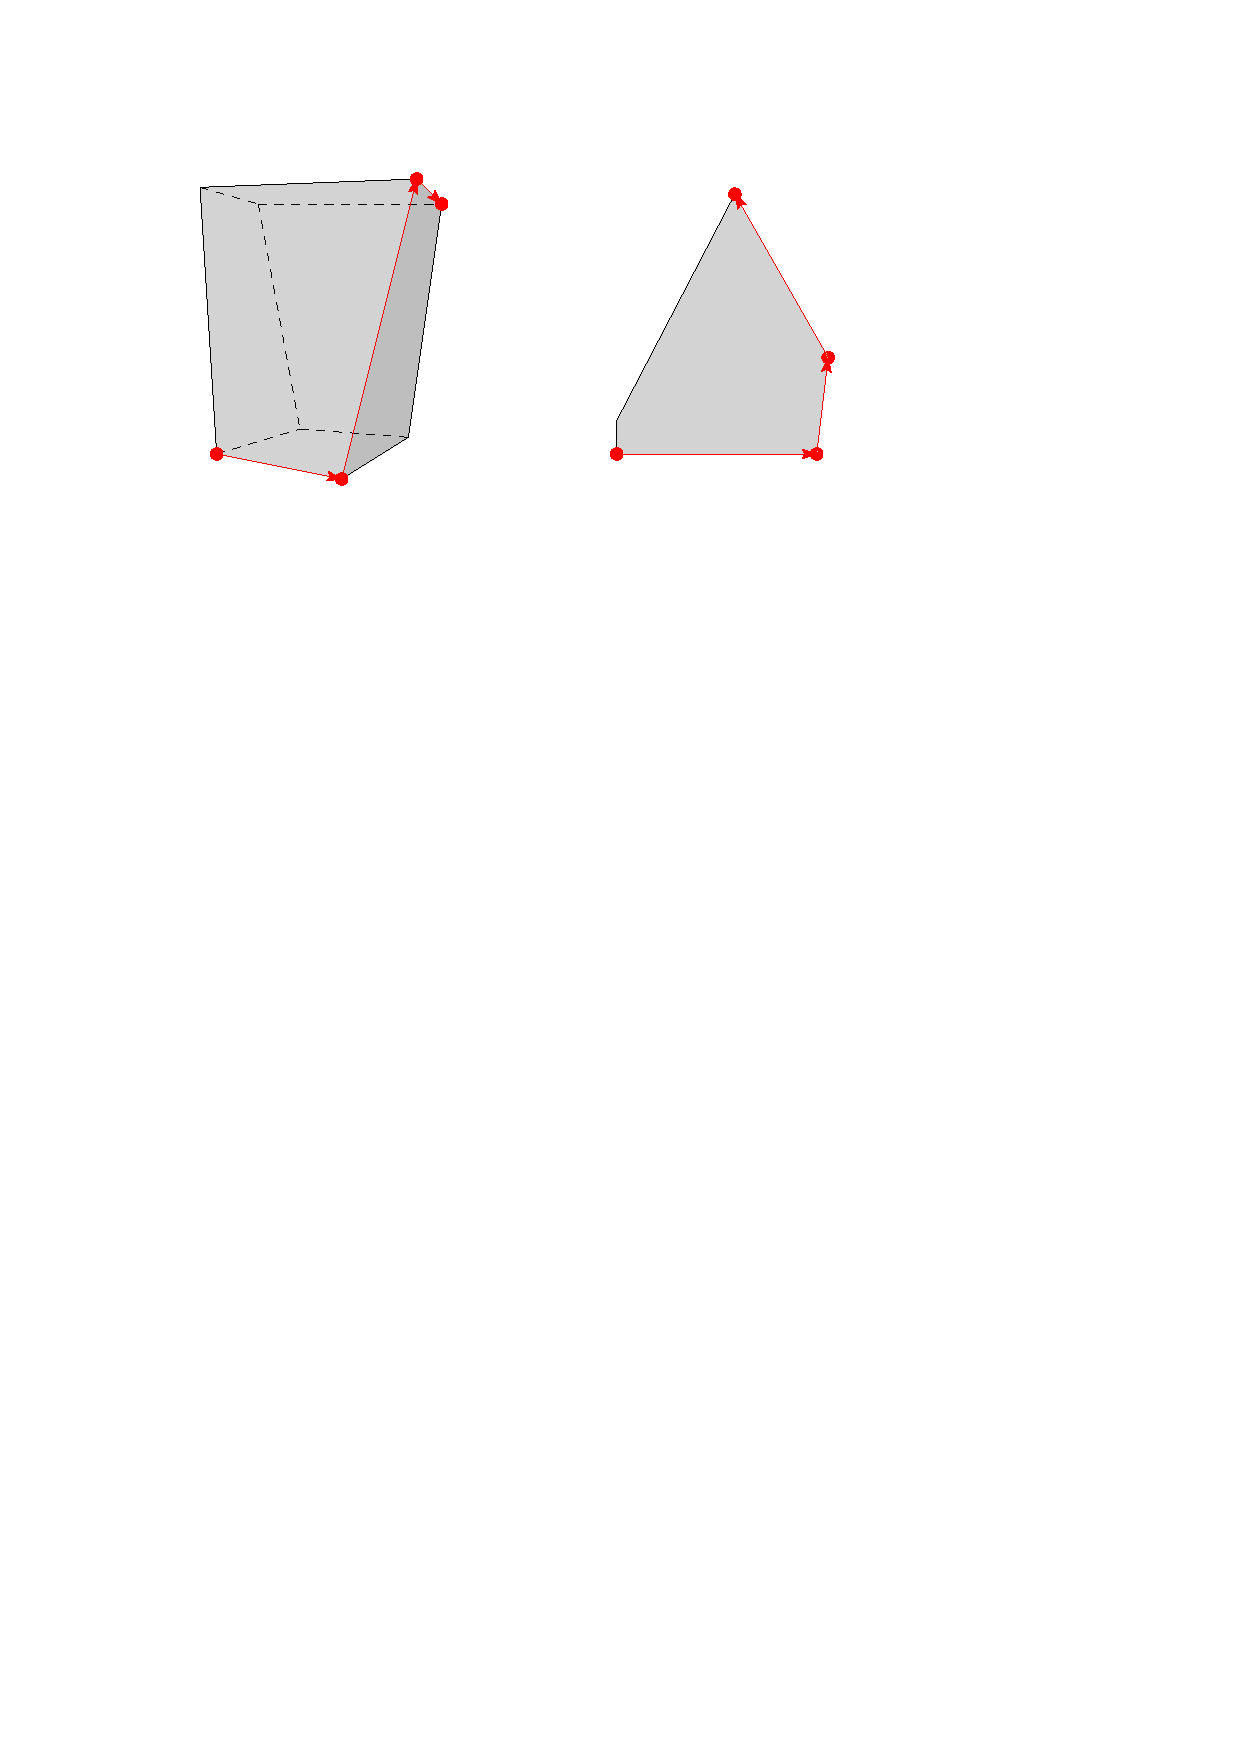
\includegraphics[width=0.5\linewidth]{lp/simplex-geometric-2.pdf}
    \caption{The geometric intuition behinds the simplex algorithm. The figure shows the simplex algorithm trying to find the optima on a 3-dimensional and 2-dimensional polytope.}
    \label{fig:simplex-geometric}
\end{figure}

\section{Pivoting}

The way the simplex algorithm navigates through the polytope and jumps between vertices in through an operation called \textbf{pivoting}.

During pivoting, we select a non-basic variable $x_e$ as the \textbf{entering variable}, and a basic variable $x_l$ as the \textbf{leaving variable}. The pivot operation switches the roles of the entering and leaving variable. $x_e$ becomes a new basic variable, and $x_l$ becomes a non-basic variable. Because of this, we also need to update the expression of other basic variables as well as the objective function. Geometrically, this corresponds to following an edge of the feasible to a neighboring vertex.

Pivoting not only affects the entering and leaving variables. Because it changes the roles of the variables, we need to update the entire linear program so that $x_e$ no longer appears as a non-basic variable in any expressions. Similarly, we also want $x_l$ to appear as a non-basic variable in every expressions. Such updates also need to be applied to the objective function.

\subsection{Update Coefficient Matrix for the Entering Variable}

Suppose we have selected $x_e$ as the entering variable and $x_l$ as the leaving variable. Currently, $x_e$ is a non-basic variable, and $x_l$ is a basic variable where
$$
x_l = b_l - a_{l1}x_1 - \cdots - a_{lj}x_j - a_{le}x_e
$$
Move the entering variable to the left-hand side and move the leaving variable to the right-hand side.
$$
a_{le}x_e = b_l - a_{l1}x_1 - \cdots - a_{lj}x_j - x_l
$$
Divide both sides by $a_{le}$, the coefficient of the entering variable.
$$
x_e = \frac{b_l}{a_{le}} - \frac{a_{l1}}{a_{le}}x_1 - \cdots - \frac{a_{lj}}{a_{le}}x_j - \frac{1}{a_{le}}x_l
$$
Now, $x_e$ has become a basic variable, and $x_l$ has become a non-basic variable.

\subsection{Update Coefficient Matrix for Other Basic Variables}

Since we have made $x_e$ a basic variable, expressed in terms of the non-basic variables, we need to update the expressions of the remaining basic variables to reflect this change.

Consider the $i$th basic variable $x_i$, with the expression
$$
x_i = b_1 - a_{i1}x_1 - \cdots - a_{ij}x_j - a_{ie}x_e
$$
We can substitute $x_e$ with its new expression in terms of the non-basic variables
$$
x_i = b_1 - a_{i1}x_1 - \cdots - a_{ij}x_j - a_{ie}\left( \frac{b_l}{a_{le}} - \frac{a_{l1}}{a_{le}}x_1 - \cdots - \frac{a_{lj}}{a_{le}}x_j - \frac{1}{a_{le}}x_l \right) 
$$
Combine like terms.
$$
x_i = \left( b_i - a_{ie}\frac{b_l}{a_{le}} \right) - \left( a_{i1}-a_{ie}\frac{a_{l1}}{a_{le}} \right) x_1 - \cdots - \left( a_{ij}-a_{ie}\frac{a_{lj}}{a_{le}} \right) x_j - \left( -a_{ie}\frac{1}{a_{le}} \right) x_l
$$

\subsection{Update Objective Function}

The objective function
$$
z = v + \sum_{j=1}^n c_j x_j
$$
also needs to be updated.

In particular, we will substitute $x_e$ with its new expression in terms of the non-basic variables. This is similar to how we update the basic variables.
$$
z = v + c_1x_1 + \cdots + c_j x_j + c_e \left( \frac{b_l}{a_{le}} - \frac{a_{l1}}{a_{le}}x_1 - \cdots - \frac{a_{lj}}{a_{le}}x_j - \frac{1}{a_{le}}x_l \right)
$$
Again, we combine like terms, yielding
$$
z = \left( v + c_e \frac{b_l}{a_{le}} \right) + \cdots + \left( c_j - c_e \frac{a_{lj}}{a_{le}} \right) x_j + \left( - c_e \frac{1}{a_{le}} \right)x_l
$$

\subsection{Pivoting Algorithm}

Based on our derivation above, we can implement the pivot operation as follows. The procedure \proc{Pivot} takes in the tuple $(N,B,A,b,c,v)$ representing a linear program in slack form, along with the index of the leaving and entering variables $l$ and $e$, and outputs a new tuple $(\hat{N},\hat{B},\hat{A},\hat{b},\hat{c},\hat{v})$.

Recall that $N$ is the set of indices of the non-basic variables, $B$ is the set of indices of the basic variables, $A$ is the coefficient matrix, $b$ and $c$ are column vectors. In the algorithm, we assume we can access the $i,j$-entry of a matrix $A$ using $a_{ij}$ representing the linear program after pivoting.

\begin{codebox}
    \Procname{$\proc{Pivot}(N,B,A,b,c,v,l,e)$}
    \li \Comment{Initialize $m \times n$ matrix}
    \li $\hat{A} = [[]]$
    \li \Comment{Calculate coefficients for new basic variable $x_e$}
    \li $\hat{b}_e = b_l/a_{le}$
    \li \For $j \in N - \{e\}$ \Do
        \li $\hat{a}_{ej} = a_{lj}/a_{le}$
    \End
    \li $\hat{a}_{el} = 1/a_{le}$
    \li \Comment{Calculate coefficients for the remaining constraints}
    \li \For $i \in B - \{l\}$ \Do
        \li $\hat{b}_i = b_i - a_{ie} \hat{b}_e$
        \li \For $j \in N - \{e\}$ \Do
            \li $\hat{a}_{ij} = a_{ij} - a_{ie} \hat{a}_{ej}$
        \End
        \li $\hat{a}_{il} = -a_{ie} \hat{a}_{el}$
    \End
    \li \Comment{Calculate the new objective function}
    \li $\hat{v} = v + c_e \hat{b}_e$
    \li \For $j \in N - \{e\}$ \Do
        \li $\hat{c}_j = c_j - c_e \hat{a}_{ej}$
    \End
    \li $\hat{c}_l = -c_e \hat{a}_{el}$
    \li \Comment{Update new sets of basic and non-basic variables}
    \li $\hat{N} = N - \{e\} \cup \{l\}$
    \li $\hat{B} = B - \{l\} \cup \{e\}$ 
    \li \Return $(\hat{N},\hat{B},\hat{A},\hat{b},\hat{c},\hat{v})$ 
\end{codebox}

\section{Simplex Algorithm}

\subsection{Basic Feasible Solution}

The simplex algorithm follows the intuitive that we have developed throughout the chapter. We start from a vertex (say, the origin) keep moving to a neighboring vertex if such move can increase the value of the objective function. We have seen that this can be done through the pivot operation. To make this idea more concrete, let's define a basic solution and a basic feasible solution.

\begin{definition}[Basic Solution] \index{basic solution}
    A solution $\mathbf{x}$ of $\mathbf{A}\mathbf{x} = \mathbf{b}$ is a \textbf{basic solution} if the set $\{ \mathbf{a}_i \mid x_i \neq 0 \}$ (the columns of $A$ corresponding to a non-zero variable) is linearly independent. Equivalently, this means that there are $n$ linearly independent constraints.
\end{definition}

\begin{definition}[Basic Feasible Solution] \index{basic feasible solution}
    A basic solution that is also a feasible solution is called a basic feasible solution.
\end{definition}

In slack form, a basic solution can be obtained by setting all non-basic variables to 0.

The goal of the simplex algorithm is to, in each iteration, reformulate the linear program so that the basic solution leads to a greater objective value. This is done by selecting the tightest basic variable as the leaving variable, a non-basic variable whose coefficient in the objective function is positive as the entering variable, and performing the pivot operation.

\subsection{Example of Simplex Algorithm}

As an example, let's examine the linear program on page 865 of CLRS.
\[
    \begin{aligned}
        \text{maximize \quad } & 3x_1 + x_2 + 2x_3 \\
        \text{subject to \quad } &x_1 + x_2 + 3x_3 &\leq 30 \\
        &2x_1 + 2x_2 + 5x_3 &\leq 24 \\
        &4x_1 + x_2 + 2x_3 &\leq 36 \\
        &x_1, x_2, x_3 &\geq 0
    \end{aligned}
\]
Convert it to slack form
\[
    \begin{aligned}
        \text{maximize \quad }  z &= 3x_1 + x_2 + 2x_3 \\
        \text{such that \quad } x_4 &= 30 - x_1 - x_2 - 3x_3 \\
        x_5 &= 24 - 2x_1 - 2x_2 - 5x_3 \\
        x_6 &= 36 - 4x_1 - x_2 - 2x_3 \\
        & x_1, x_2, x_3, x_4, x_5, x_6 \geq 0
    \end{aligned}
\]
Set all non-basic variables $x_1,x_2,x_3$ to 0 and obtain the basic solution $x_1=0,\,x_2=0,\,x_3=0,\,x_4=30,\,x_5=24,\,x_6=36$. The objective value for this basic solution is 0. (Starts from the origin of the feasible region.)

Select $x_1$ as entering variable because it has a positive coefficient in the objective function. The tightest constraint is $x_6$ since $x_1$ can only increase by 9 while maintaining $x_6 \geq 0$. Perform pivot operation, and we get
\[
    \begin{aligned}
        \text{maximize \quad }  z &= 27 + \frac{x_2}{4} + \frac{x_3}{2} - \frac{3x_6}{4} \\
        \text{such that \quad } x_1 &= 9 - \frac{x_2}{4} - \frac{x_3}{2} - \frac{x_6}{4} \\
        x_4 &= 21 - \frac{x_2}{4} - \frac{x_3}{2} - \frac{x_6}{4} \\
        x_5 &= 6 - \frac{3x_2}{2} - 4x_3 + \frac{x_6}{2} \\
        & x_1, x_2, x_3, x_4, x_5, x_6 \geq 0
    \end{aligned}
\]
The basic solution is currently $x_1=9,\,x_2=0,\,x_3=0,\,x_4=21,\,x_5=6,\,x_6=0$ with $z=27$. Select $x_3$ as the next entering variable. $x_5$ has the tightest constraint, so $x_5$ is the leaving variable. Perform pivot operation.
\[
    \begin{aligned}
        \text{maximize \quad }  z &= \frac{111}{4} + \frac{x_2}{16} - \frac{x_5}{8} - \frac{11x_6}{16} \\
        \text{such that \quad } x_1 &= \frac{33}{4} - \frac{x_2}{16} + \frac{x_5}{8} - \frac{5x_6}{16} \\
        x_3 &= \frac{3}{2} - \frac{3x_2}{8} - \frac{x_5}{4} + \frac{x_6}{8} \\
        x_4 &= \frac{69}{4} + \frac{3x_2}{16} - \frac{5x_5}{8} - \frac{x_6}{16} \\
        & x_1, x_2, x_3, x_4, x_5, x_6 \geq 0
    \end{aligned}
\]
The basic solution is currently $x_1=\frac{33}{4},\,x_2=0,\,x_3=\frac{3}{2},\,x_4=\frac{69}{4},\,x_5=0,\,x_6=0$ with $z=\frac{111}{4}$. Select $x_2$ as the next entering variable as it is the only variable with a positive coefficient in the objective function. $x_3$ has the tightest constraint while $x_4$ puts no constraint on how much we can increase $x_2$. $x_3$ will be the next leaving variable.
\[
    \begin{aligned}
        \text{maximize \quad }  z &= 28 - \frac{x_3}{6} - \frac{x_5}{6} - \frac{2x_6}{3} \\
        \text{such that \quad } x_1 &= 8 + \frac{x_3}{6} + \frac{x_5}{6} - \frac{x_6}{3} \\
        x_2 &= 4 - \frac{8x_3}{3} - \frac{2x_5}{3} \frac{x_6}{3} \\
        x_4 &= 18 - \frac{x_3}{2} + \frac{x_5}{2} + 0x_6 \\
        & x_1, x_2, x_3, x_4, x_5, x_6 \geq 0
    \end{aligned}
\]
Observe that at this stage, none of the nonbasic variables in the objective function has positive coefficient, so it cannot be optimized anymore. The optimal solution to the original linear program is $x_1=8,x_2=4,x_3=0$ with $z=28$.

Going back to our geometric intuition for the simplex algorithm, the algorithm can be understood as follows. We start from the origin $(0,0,0)$. Increase $x_1$ until it hits the barrier set forth by $x_6$ (tightest constraint). Increase $x_3$ until it hits the barrier set forth by $x_5$ (tightest constraint). Increase $x_2$ until it hits the barrier by $x_3$ (tightest constraint). Indeed, just as described in our geometric interpretation, the simplex algorithm travels along the edges of the feasible region to neighboring vertices and finds an optimal solution at one of vertices of the feasible region. See Figure \ref{fig:simplex-example}.

\begin{figure}[htbp]
    \centering
    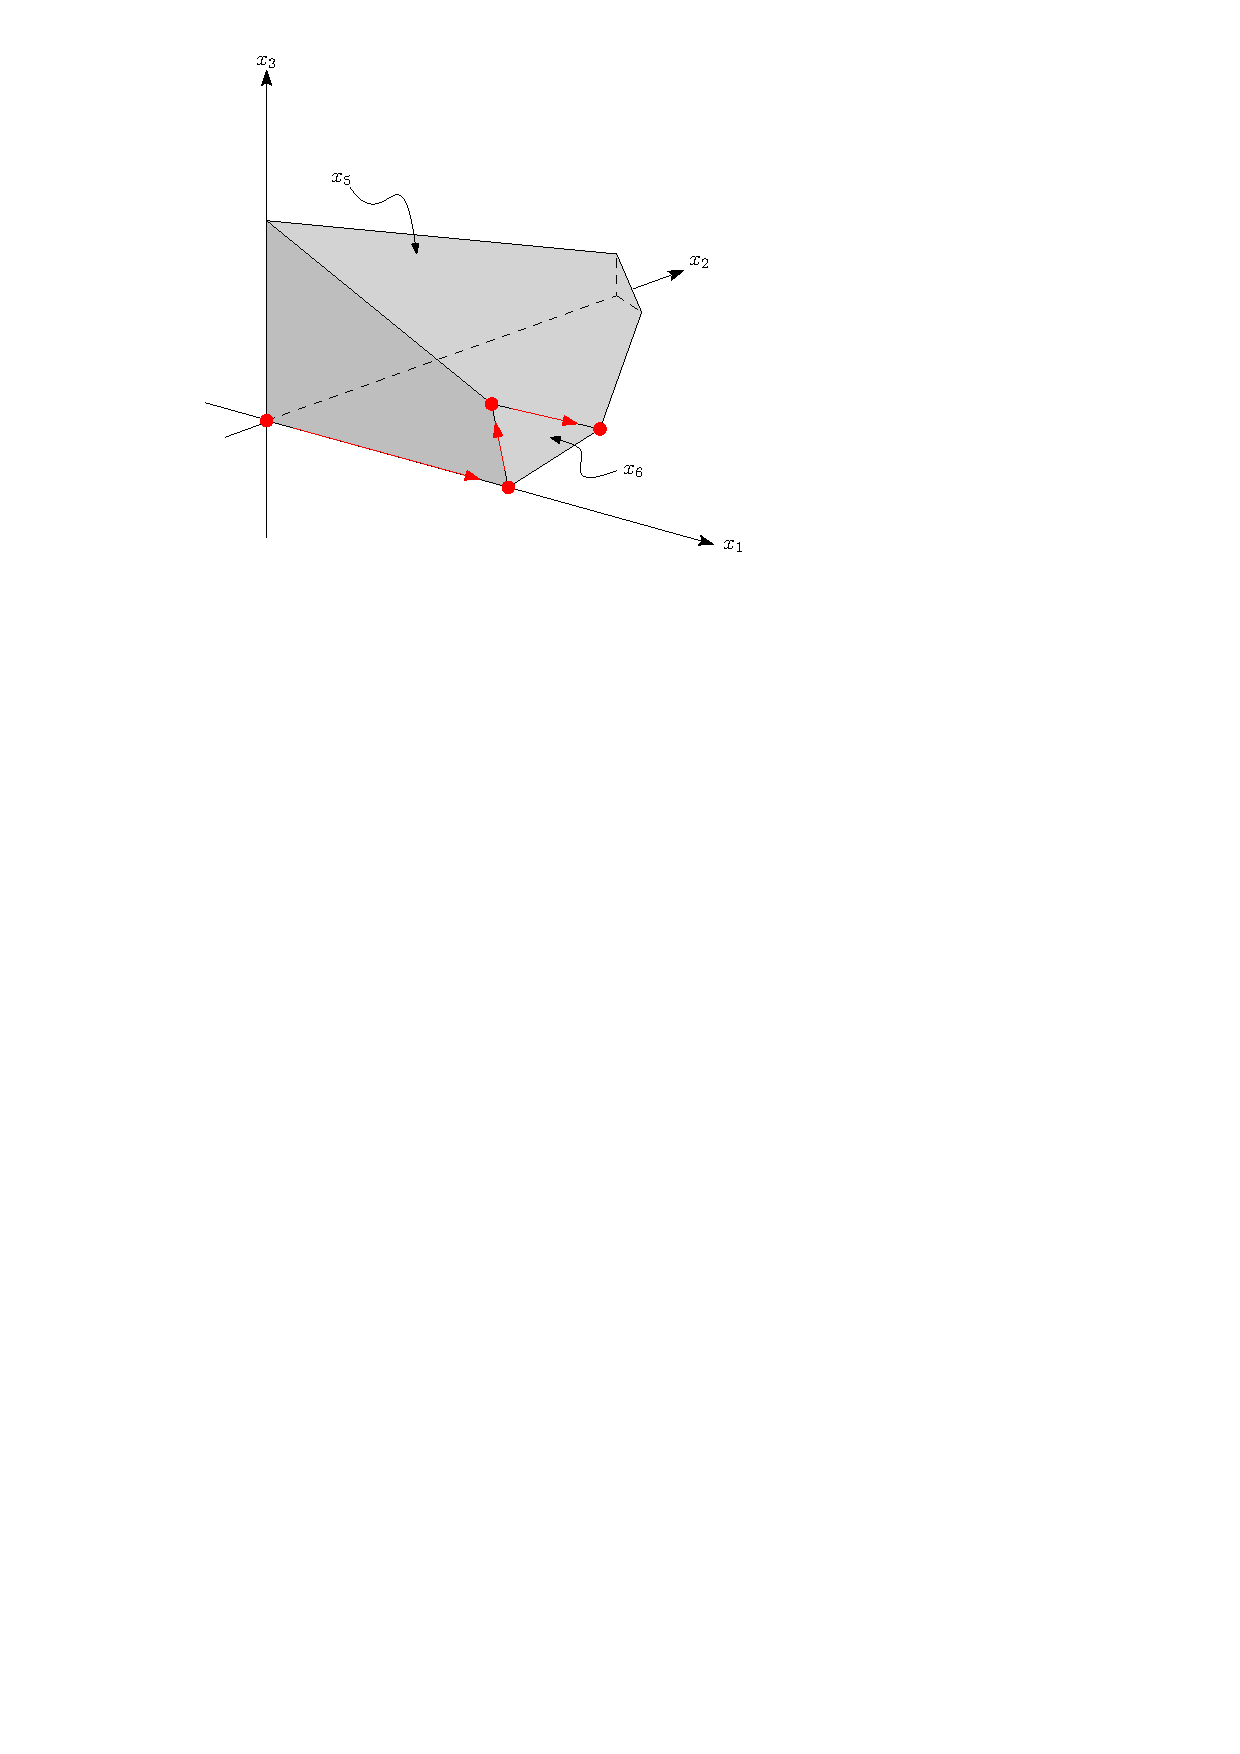
\includegraphics[width=0.4\linewidth]{lp/simplex-example-3d.pdf}
    \qquad\qquad
    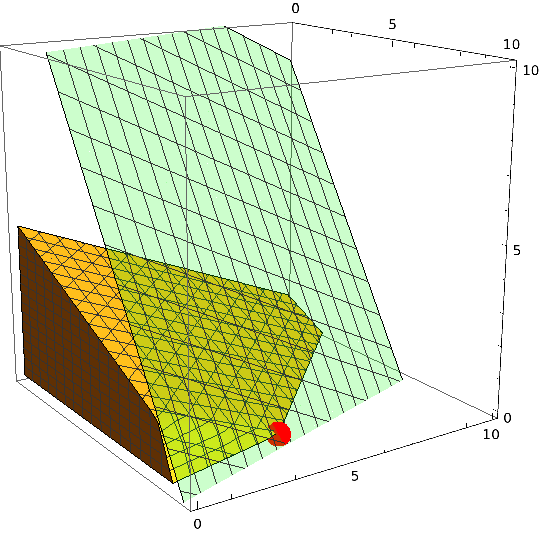
\includegraphics[width=0.4\linewidth]{lp/simplex-example-3d-2.pdf}
    \caption{Running the simplex algorithm on the example linear program. The figure on the right shows the feasible region in orange with the objective function as a green plane, and the optimum as a red dot in the graph.}
    \label{fig:simplex-example}
\end{figure}

\subsection{Finding the Tightest Constraint}

The tightest constraint can be easily identified using a method known as the \textbf{minimum ratio test}. Once we have selected a non-basic variable as entering variable, say $x_e$, we iterate over the basic variables, and select the $i$th basic variable that minimizes $b_i/a_{ie}$ if $a_{ie}$ is negative. If $a_{ie}$ is positive, then the constraint does not limit how much we can increase $x_e$. In more concise notation, 
$$
l = \Argmin_{i \in \{b \in B \mid a_{be} > 0\}} \frac{b_i}{a_{ie}}.
$$
This should be quite intuitive. Consider the expression of a basic variable with nonnegativity constraint of the form
$$
x_i = b_i - a_{i1} x_1 - \cdots - a_{ie} x_e \geq 0
$$
$x_e$ is bounded by $b_i/a_{ie}$, so to find the tightest constraint on how much we can increase $x_e$, we want to minimize the ratio $b_i/a_{ie}$.

\subsection{Implementing the Simplex Algorithm}

\section{Time Complexity of the Simplex Algorithm}

